\documentclass[12pt]{article}       %{amsart}

\usepackage[svgnames]{xcolor} 

\usepackage{amsmath, amsthm, ulem, graphicx, marvosym, fancyhdr, amscd, amssymb, float, enumerate}

%added as part of article format

\topmargin -.3in
\evensidemargin -.1in
\oddsidemargin -.1in
\textheight 8.5in
\textwidth 6.5in
\def\hs{\hspace{15pt}}

\newcommand*{\titleAT}{\begingroup % Create the command for including the title page in the document
\newlength{\drop} % Command for generating a specific amount of whitespace
\drop=0.1\textheight % Define the command as 10% of the total text height

\rule{\textwidth}{1pt}\par % Thick horizontal line
\vspace{2pt}\vspace{-\baselineskip} % Whitespace between lines
\rule{\textwidth}{0.4pt}\par % Thin horizontal line

\vspace{\drop} % Whitespace between the top lines and title
\centering % Center all text
\textcolor{Red}{ % Red font color
{\Huge Pew Pew: A Two-Dimensional Space Shooter Game with Roguelike Gameplay Mechanics}\\[0.5\baselineskip] % Title line 1
%{\Large with}\\[0.75\baselineskip] % Title line 2
{\Huge }} % Title line 3

\vspace{0.25\drop} % Whitespace between the title and short horizontal line
\rule{0.3\textwidth}{0.4pt}\par % Short horizontal line under the title
\vspace{\drop} % Whitespace between the thin horizontal line and the author name

{\Large \textsc{George Bateman BS CS \\* Jacob Cannon BS CS \\* Nicholas DeVoll BS CS \\* \vspace{3pt} Madison Silva BA CS}}\par % Author name

\vfill % Whitespace between the author name and publisher text

{\large \textsc{Faculty Mentor: Dr. Jorge Reyes Silveyra}}\par 

{\large \textsc{May 15th 2015}}\par

\vspace*{\drop} % Whitespace under the publisher text

\rule{\textwidth}{0.4pt}\par % Thin horizontal line
\vspace{2pt}\vspace{-\baselineskip} % Whitespace between lines
\rule{\textwidth}{1pt}\par % Thick horizontal line

\endgroup}

\setcounter{tocdepth}{2}

\begin{document}

\begin{titlepage}
\thispagestyle{empty}
\titleAT
\end{titlepage}

\newpage
\begin{titlepage}
\thispagestyle{empty}
\tableofcontents
\end{titlepage}

\begin{titlepage}
\thispagestyle{empty}
\listoffigures
\end{titlepage}

%\author{Madison Silva}\address{Pacific Lutheran University\\ Tacoma, WA 98447}%\email{silvamj@plu.edu}

\newpage

\begin{abstract} We examine the implementations of various enemies, weapons, and game behavior in our two dimensional space shooter. Among them are systems such as shooting predictively at the player, swapping weapons using wrappers, and utilizing Unity prefabs.
\end{abstract}

\section{Introduction} %INTRODUCTION 
\label{sec:intro}

\hs Video games have been a rapidly growing industry in the past 30 years \cite{History}. As such, there are a wide variety of genres and subgenres of games, each taking influence from and building upon successful games of the past. In some cases these games combine past elements in a way that create a new category of game. The goal of this project is to develop a game that will blend space-shooter elements from classic arcade games, such as Asteroids and Galaga, with randomized, challenging elements from more recent games such as The Binding of Isaac. These elements include random pick-ups, permanent player death, and semi-random wave spawning. This combinationl aims to provide players with new challenges that may not be available in current games. This game was developed using Unity3D andl runs in the Unity engine, which features robust tools that allowed us to manipulate nearly any element of the game quickly and with immediate feedback.

\subsection{Basic Unity Features} % Need to talk about prefabs and other Unity functionality: Layer, Camera, Scene, Hierarchy, Prefab
\begin{figure} [H]
\centering
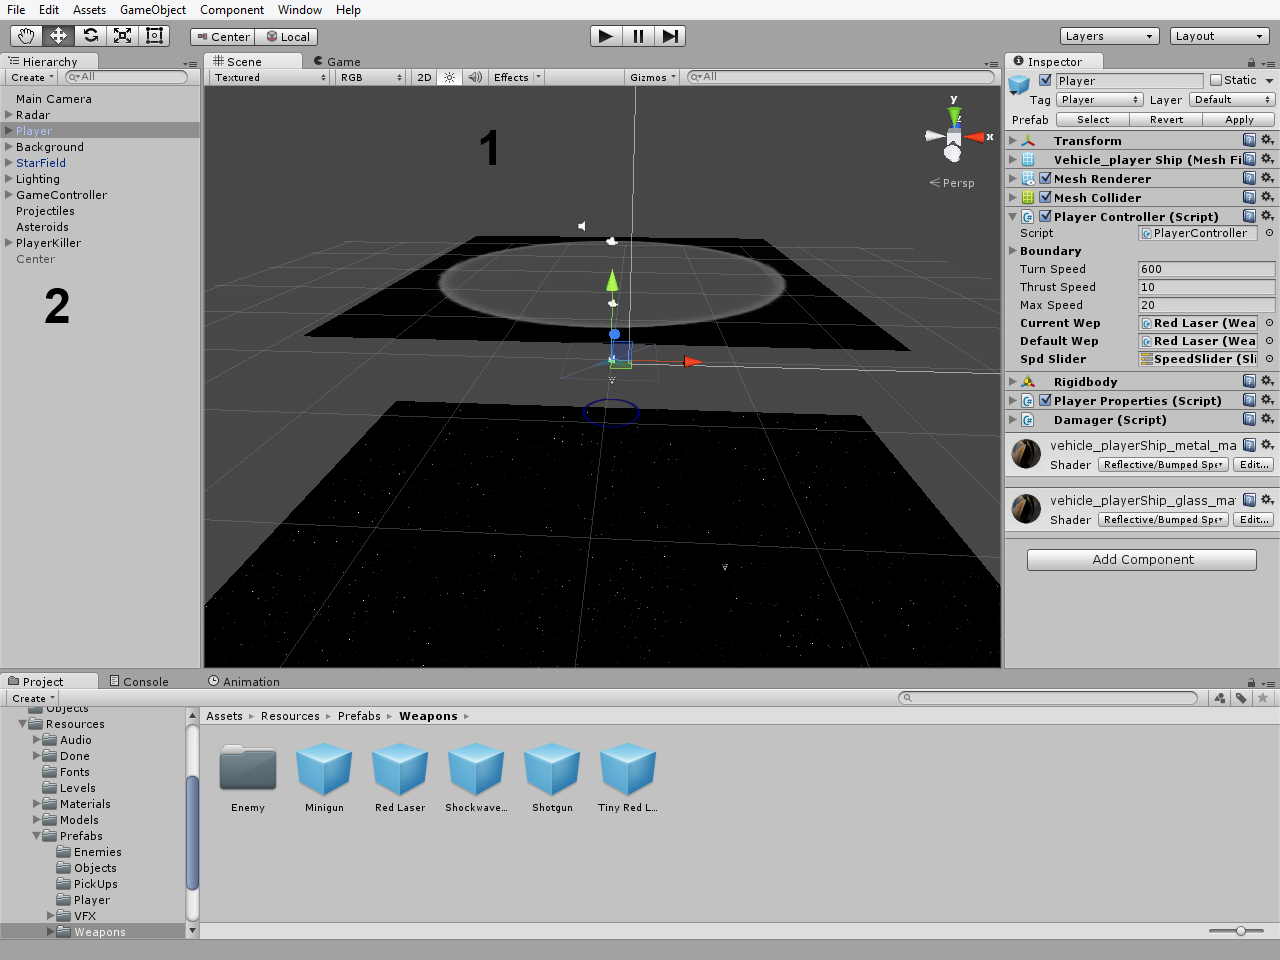
\includegraphics[width=7in]{scene.png}
\caption{Unity Editor} \label{Unity}
\end{figure}

\hs {\bf Scene:} The scene view, shown in the middle of Figure \ref{Unity}, shows where all of the Unity objects are inside the current level. Scenes are independent from each other and moving from one scene to another loads an entirely new level with new scripts, objects, etc.

{\bf Hierarchy:} The object hierarchy, seen in the top left of Figure \ref{Unity}, shows how the game objects are laid out inside the current scene. Game objects use a parent/child relationship as defined in the object hierarchy.

{\bf Camera:} A camera in Unity renders what it "sees" in front of itself to the screen, much like a normal camera would. Cameras can be adjusted in the scene view of the editor.

{\bf Layer:} A layer in Unity defines what is actually rendered to the camera. If an object is on a different layer than the camera's layer, the camera will not render it.

{\bf Prefab:} A prefab is a saved instance of a game object which can then be loaded as either a child of a game object or its own instance. Any game object can be saved as a prefab.

\subsection{Background}
	For the development of this project, we will develop a video game using Unity. The majority of the research time will be used to learn the functionality of Unity. Since Unity is a complete game engine and editor, the game creation process will not require the development of an engine. Other alternative engines, such as the graphics engine Ogre3D, would still require the implementation of a game engine in addition to creating the game \cite{Ogre}. Unreal Engine 4 was another considered engine, and included many features that would be useful to this project. However, many individuals have said that it is difficult for beginners to learn due to the lack of tutorials. Ultimately, we settled on Unity, since it has a wide range of tutorials to help us get started more quickly and will allow the majority of the project resources to go towards gameplay. development.

        Unity primarily uses $C\#$ as it’s scripting language. $C\#$ was created by Microsoft in 1997. It uses the .NET framework and is the most popular .NET language used today. It was influenced heavily by Java and C++, and it is intended to be friendly to the software development process so it has features such as uninitialized variable compatibility and automatic garbage collection \cite{Cadet}. Even though $C\#$ is a compiled language, Unity is still able to use $C\#$ code snippets as “scripts” because Unity is built in IDE (Monodevelop), compiles the code and packages it with game resources before runtime. This gives the games a robust set of tools, but allows the game to load and run quickly. \cite{Moles} 

	Our game strives to follow the principles set out by previous roguelike games. The term roguelike is a broad term used to describe video games that use random elements to create a replayable game that restarts the player on each subsequent playthrough. The original game that spawned this categorization was the game Rogue. Rogue was programmed at UC Santa Cruz in the 1980’s, using ASCII characters to take players on an adventure through a subterranean dungeon for the Amulet of Yendor. Once the game was released to others outside the developer, it spread rapidly throughout the college and the surrounding communities. Rogue inspired many other hits in the video game industry, including Diablo II, Faster Than Light, and The Binding of Isaac. \cite{Rogue}

	While developing non-player entities it is crucial to have an AI. Without an AI the entity becomes a stationary object and if they are an enemy that is not very exciting. One of the first step in creating a basic AI is choosing a pathfinding algorithm, so that the entity will move properly. An example of a basic but effective pathfinding algorithm is A*. Amit Patel defines A* as a combination of Dijkstra’s Algorithm and the Best-First-Search Algorithm \cite{A}. Dijkstra’s Algorithm searches all cells around the starting point moving out and searching the next farthest out cells in each direction until it finds the goal. In a game where time is valuable searching in the way would be inefficient. Best- First-Search(BFS) is faster because it searches only in the direction of the goal. This algorithm is not efficient for games because if there is an obstacle then the path that BFS takes can become inefficient. A* searches all vertices by favoring the ones in the direction of the goal, this helps it be more efficient like BFS but avoid obstacles more like Dijkstra’s. \cite{A}

	Finally, procedurally generated content will be used in order to build satisfying and challenging areas for the player. Procedural content generation is the process of designing an algorithm that can generate content at runtime. This fits in well with this project. With a relatively small number of inputs, the game can generate numerous different levels where the enemies encountered are found in different combinations. It also embodies the core idea of a roguelike game, changing the game every playthrough to challenge the player differently. There are a multitude of content generation algorithms, one of the common ones being Perlin noise, which actually refers to two algorithms created by Ken Perlin. These algorithms use a sum of different functions with varying amplitudes and frequencies in order to generate what is called a noise function. It is this function that is used to define different points of intensity. As it pertains to this project, these functions could be used to generate nebulae or star maps, giving a different visual experience to our player every time. \cite{PCG}


\section{Gameplay} %GAMEPLAY
\label{sec:Gameplay}

{\bf First Minute: } The player enters the game in their ship, and can immediately start exploring the area in which they spawn. The player is given a few moments to get used to the controls before the first wave spawns. In this first wave, only a few enemies will be created at the other side of the field. The player must find and defeat these enemies to clear the field and move on to the next wave. 

{\bf Gameflow:} 


{\bf Victory conditions}: The player will achieve victory by defeating all of the enemies in each wave that is generated without dying. The game culminates with a boss fight, and defeating this boss will trigger victory menu and end the game.

\section{Requirements} %REQUIREMENTS
\label{sec:Requirements}

\hs The following use cases and diagrams describe how the game will be implemented in the Unity game engine. While Unity is set up to handle the View portion and some of the Controller portion of the MVC architecture, we will have to supply part of the Controller and the Model portion in order to deliver our game.

\subsection{Use Case Scenarios} 
%%%
Scenario Name: {\bf PlayerDeath} \\
Participating Actor Instances:        \hspace{46pt} {\bf Player: PlayerEntity

					          \hspace{2.6 in}   Damager: DamageEntity 

					          \hspace{2.6in}    Heath: PlayerHP

						\hspace{2.6in}   Shield: PlayerShield} \vspace{10pt}  \\ 
Flow of Events: 
\begin{enumerate} 
\item {\bf Player }collides with {\bf DamageEntity}.
       \item {\bf PlayerShield} decreases based on DamageEntity. 
       \item {\bf PlayerHP} decreases based on DamageEntity and Shield. 
                \begin{enumerate}[a.]
                 \item {\bf PlayerHP} is greater than zero, continue as normal.
                 \item{\bf PlayerHP} is less than or equal to zero, {\bf Player} dies.
                      \begin{enumerate}[i.]
                	\item {\bf Player} is deleted.
                	\item Explosion animation spawned in place of {\bf Player}.
		\item An end game menu prompts {\bf Player} to either play again or return to main menu.
		 \end{enumerate}
                \end{enumerate}
\end{enumerate}

%%%
\begin{center} \line(1,0){350} \end{center}
Scenario Name: {\bf GameComplete} \\
Participating Actor Instances:        \hspace{46pt} {\bf Player: PlayerEntity

					          \hspace{2.6 in}   Boss: HostileEntity 

                                                      \hspace{2.6 in}   Bullet: Projectile} \vspace{10pt}  \\ 
Flow of Events: 
\begin{enumerate} 
\item {\bf Boss} is destroyed by a {\bf Bullet} shot by the {\bf Player}.
\item {\bf Boss} will enter an animation where it explodes.
\item {\bf Player} enters  a five second grace period where they must survive.
	\begin{enumerate} [a.]
	\item {\bf Player} does not survive the grace period and dies, restarting the game.
	\item {\bf Player} survives the grace period.
		\begin{enumerate} [i.]
		\item {\bf Player} is treated to a victory screen.
		\item {\bf Player} is given the option to play again or quit.
		\end{enumerate}
	\end{enumerate}
\end{enumerate}

%%%
\begin{center} \line(1,0){350} \end{center}
Scenario Name: {\bf LeavingFieldOfPlay} \\
Participating Actor Instances:        \hspace{46pt} {\bf Player: PlayerEntity

					          \hspace{2.6 in}  Projectile: PlayerKiller}  \vspace{10pt}  \\ 
Flow of Events: 
\begin{enumerate} 
\item {\bf Player} leaves the field of play.
\item Warning alarm sounds, warning flashes on screen.
      \begin{enumerate}[a.]
       \item {\bf Player} chooses to turn around and return to field of play, everything returns to normal.
       \item {\bf Player} advances farther out of the field of play.
                \begin{enumerate}[i.]
                \item {\bf PlayerKiller} kills {\bf Player}.
                \end{enumerate}
        \end{enumerate}
\end{enumerate}

%%%
\begin{center} \line(1,0){350} \end{center}
Scenario Name: {\bf SpawnEnemyWave} \\
Participating Actor Instances:        \hspace{46pt} {\bf Enemy: EnemyEntity

						\hspace{2.6 in} Wave: float

					          \hspace{2.6 in}   GC: GameController}  \vspace{10pt}  \\ 
Flow of Events: 
\begin{enumerate} 
\item {\bf GC} waits a set amount of time before attempting to spawn a wave.
\item The allotted amount of time has passed.
	\begin{enumerate} [a.]
	\item {\bf Wave} is not equal to the number of total waves.
		\begin{enumerate} [i.]
		\item Enemies are spawned in according to how many waves the player has defeated.
		\end{enumerate}
	\item {\bf Wave} is equal to the number of total waves.
		\begin{enumerate} [i.]
		\item The boss is spawned in and the player must fight them to win.
		\end{enumerate}
	\end{enumerate}
\end{enumerate}

%%%
\begin{center} \line(1,0){350} \end{center}
Scenario Name: {\bf MoveAndShoot} \\
Participating Actor Instances:        \hspace{46pt} {\bf Player: PlayerEntity

					          \hspace{2.6 in}   Bullet:Projectile}  \vspace{10pt}  \\ 
Flow of Events: 
\begin{enumerate} 
\item {\bf Player} presses a movement button, which defaults to the WASD keys, while simultaneously pressing a fire button, which default to the $ \uparrow \downarrow \leftarrow \to $ arrow keys.
\item {\bf Player} moves in the direction of the movement button pressed, while {\bf Bullet} is fired in the direction of the fire button pressed.
\item {\bf Player} continues moving in the way of the first directional input until an additional input is received, at which time {\bf Player} will begin to move in the way of the second directional input. 
\item {\bf Bullet} travels in the direction it was initially shot without the possibility of changing direction.
\end{enumerate}

%%%
\begin{center} \line(1,0){350} \end{center}
Scenario Name: {\bf SpawnAsteroids} \\
Participating Actor Instances:        \hspace{46pt} {\bf Enemy: EnemyEntity

						\hspace{2.6 in} Asteroid: AsteroidEntity

						\hspace{2.6 in}  GC: GameController}  \vspace{10pt}  \\ 
Flow of Events: 
\begin{enumerate} 
\item {\bf GC} performs a check to see if an asteroid will spawn.
\item The check fails.
	\begin{enumerate} [a.]
	\item Nothing occurs, and {\bf GC} waits before attempting to spawn another.
	\end{enumerate}
\item The check passes.
	\begin{enumerate} [a.]
	\item An {\bf Asteroid} object is spawned with a random position, movement vector, and rotation speed.
	\item The {\bf Asteroid} careens through space until it hits something or goes too far away.
		\begin{enumerate} [i.]
		\item The {\bf Asteroid} is then destroyed.
		\end{enumerate}
	\end{enumerate}
\end{enumerate}

%%%
\begin{center} \line(1,0){350} \end{center}
Scenario Name: {\bf BulletFizzle} \\
Participating Actor Instances:        \hspace{46pt} {\bf Player: PlayerEntity

					          \hspace{2.6 in}   Bullet: Projectile}  \vspace{10pt}  \\ 
Flow of Events: 
\begin{enumerate} 
\item {\bf Player} shoots a {\bf Bullet}.
\item {\bf Bullet} does not hit anything within the view of the {\bf Player}.
\item {\bf Bullet} travels out of the view of the {\bf Player}.
      \begin{enumerate}[a.]
       \item The {\bf Bullet} collides with an entity
                \begin{enumerate}[i.]
                \item The {\bf Bullet} causes damage to that entity, and terminates itself.
                \end{enumerate}
      \item The {\bf Bullet} does not collide with anything.
                \begin{enumerate}[i.]
                \item The {\bf Bullet} is terminated after a short distance.
                \end{enumerate}
        \end{enumerate}
\end{enumerate}

%%%
\begin{center} \line(1,0){350} \end{center}
Scenario Name: {\bf SpawnPickUp} \\
Participating Actor Instances:        \hspace{46pt} {\bf Player: PlayerEntity
	
						\hspace{2.6 in} Enemy: EnemyEntity

					          \hspace{2.6 in}  Shotgun: PickUp}  \vspace{10pt}  \\ 
Flow of Events: 
\begin{enumerate} 
\item {\bf Player} destroys an {\bf Enemy} with its weapon.
\item {\bf Enemy} rolls a check to see if it drops anything.
\item The check succeeds, and {\bf Enemy} drops a {\bf Shotgun} pickup.
\item {\bf Player} touches the {\bf Shotgun}.
\item The {\bf Shotgun} is equipped, giving {\bf Player} 50 ammo and the {\bf Shotgun} weapon.
\end{enumerate}

%%%
\begin{center} \line(1,0){350} \end{center}
Scenario Name: {\bf PauseGame} \\
Participating Actor Instances:        \hspace{46pt} {\bf Player: PlayerEntity }  \vspace{10pt}  \\ 
Flow of Events: 
\begin{enumerate} 
\item {\bf Player} presses the pause button.
	\begin{enumerate} [a.]
	\item A screen displays over the main screen, informing the {\bf Player} the game is paused.
	\item The game's timescale is set to 0, freezing any objects currently in the scene.
	\end{enumerate}
\item {\bf Player} presses the pause button once more. 
	\begin{enumerate} [a.]
	\item The pause screen is disabled and removed.
	\item The game's timescale is set back to 1, resuming the action.
	\end{enumerate}
\end{enumerate}


\subsection{Use Case Model}
Figure \ref{Use Case Model} shows which external actors participate in each of the Use Case Scenarios included.

\begin{figure} [H]
\centering
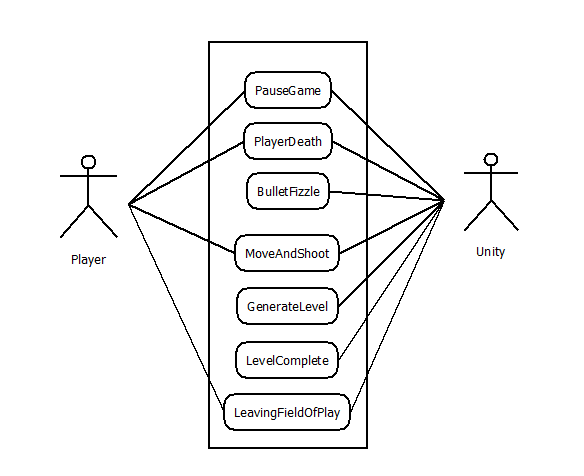
\includegraphics[width=5.5in]{UseCaseModel1.png}
\caption{Use Case Model} \label{Use Case Model}
\end{figure}


\section{Design} %DESIGN
\label{sec:Design}

\subsection{Sequence Diagram}
The sequence diagram represented in Figure \ref{PlayerDeath}  corresponds to the use case PlayerDeath, and outlines the process behind the player being hit with a projectile to a death state, followed by the appropriate response by the {\it GameController}. Health will only be subtracted if the player has no remaining shield. If the player no longer has any health or shields after taking damage, then the {\it Player} object will report its death to the {\it GameController}. Sequence diagrams for other use cases are functionally similar, albeit with a few differing actors and method calls.

\begin{figure} [H]
\centering
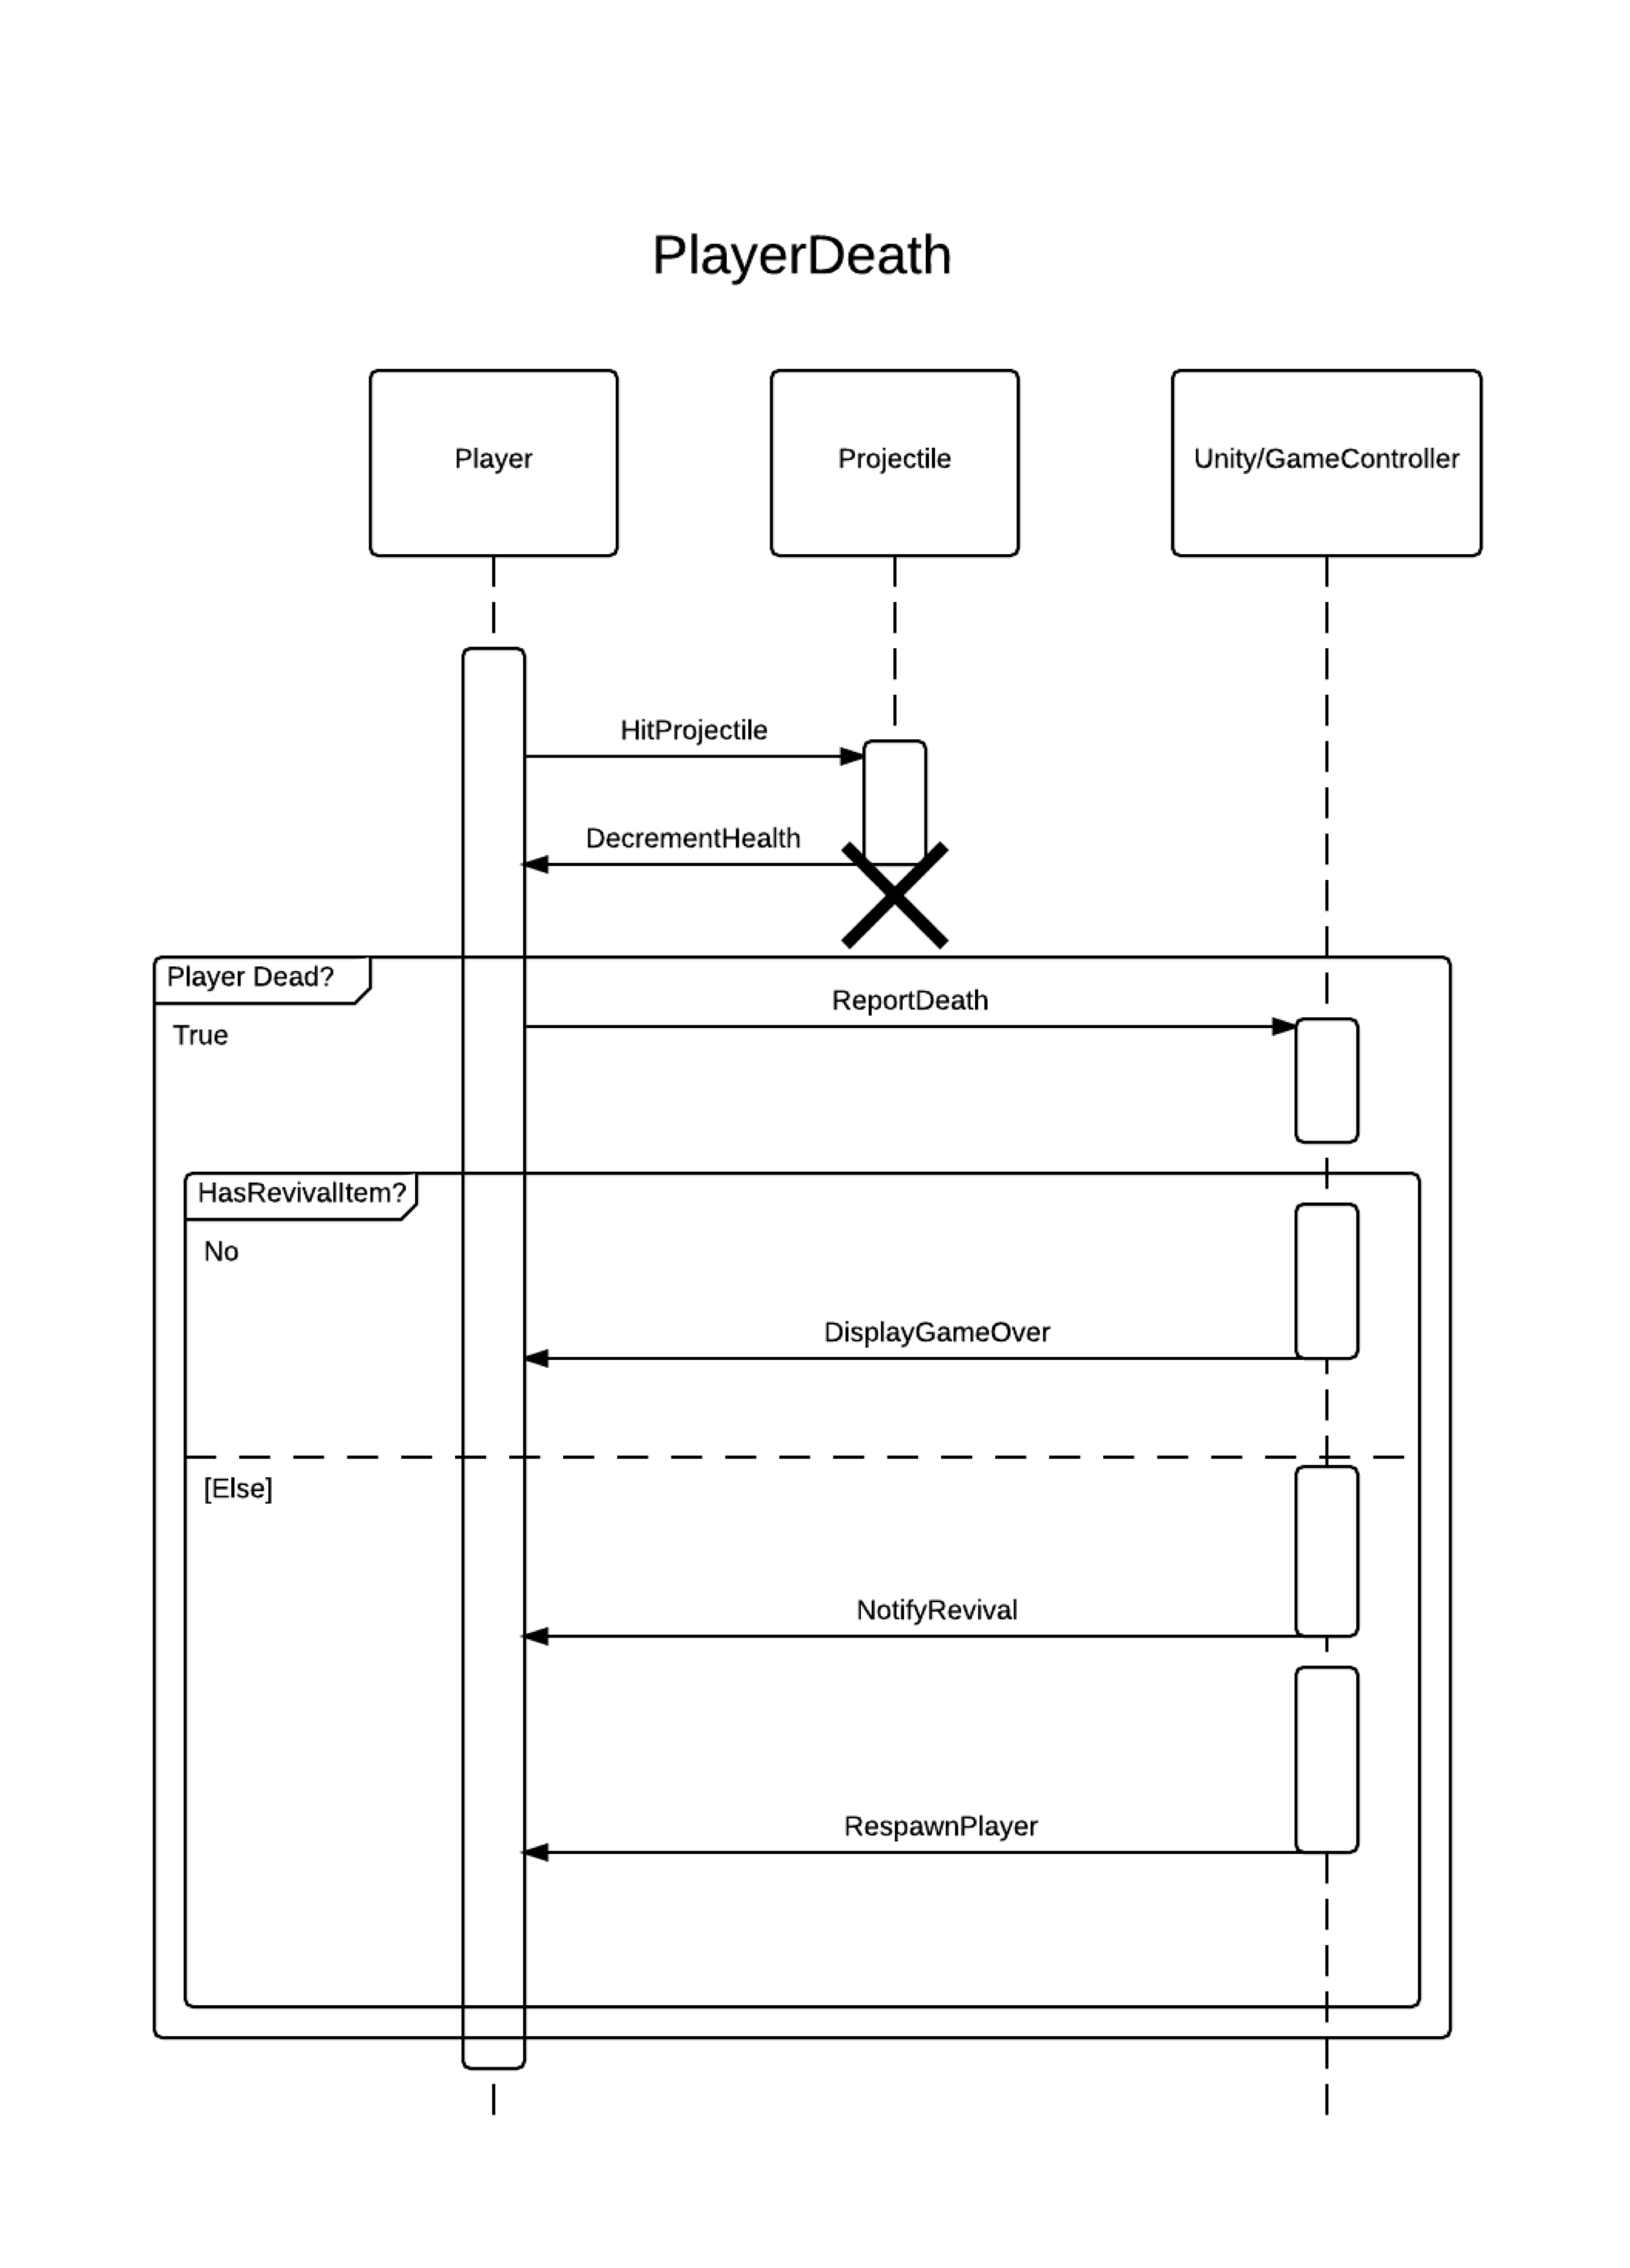
\includegraphics[width=4.75in]{PlayerDeath.png}
\caption{Player Death Sequence Diagram} \label{PlayerDeath}
\end{figure}

\subsection{UML Diagram}
\hs In Figure \ref{UML} shows the core class design for the game and the relations that classes will have with each other. Classes will be interacting with existing classes of the Unity engine. {\it GameManager} will be a singleton class that will be responsible for holding the {\it Player Entity}, this way the game can easily transport the {\it Player} between scenes without risk of creating a duplicate {\it Player}. {\it GameController} will handle everything that happens inside the level itself, and will be able to do this with the onAwake() function, provided by Unity, that activates when the script has been loaded into the scene. The {\it Entity} object will provide a basis of all entities in-game that will be able to move and react to the game state, including the {\it Player}. The {\it Ship} class will be a prefab handled by Unity that will allow us to instantiate an {\it Entity} object with certain variables from the start. Our {\it Item} and {\it Weapon} interfaces will handle items and weapons picked up in the game, respectively. It is important that there is a distinction between the two, as all {\it Weapons} are {\it Items} but not all {\it Items} are {\it Weapons}.

\begin{figure} [H]
\centering
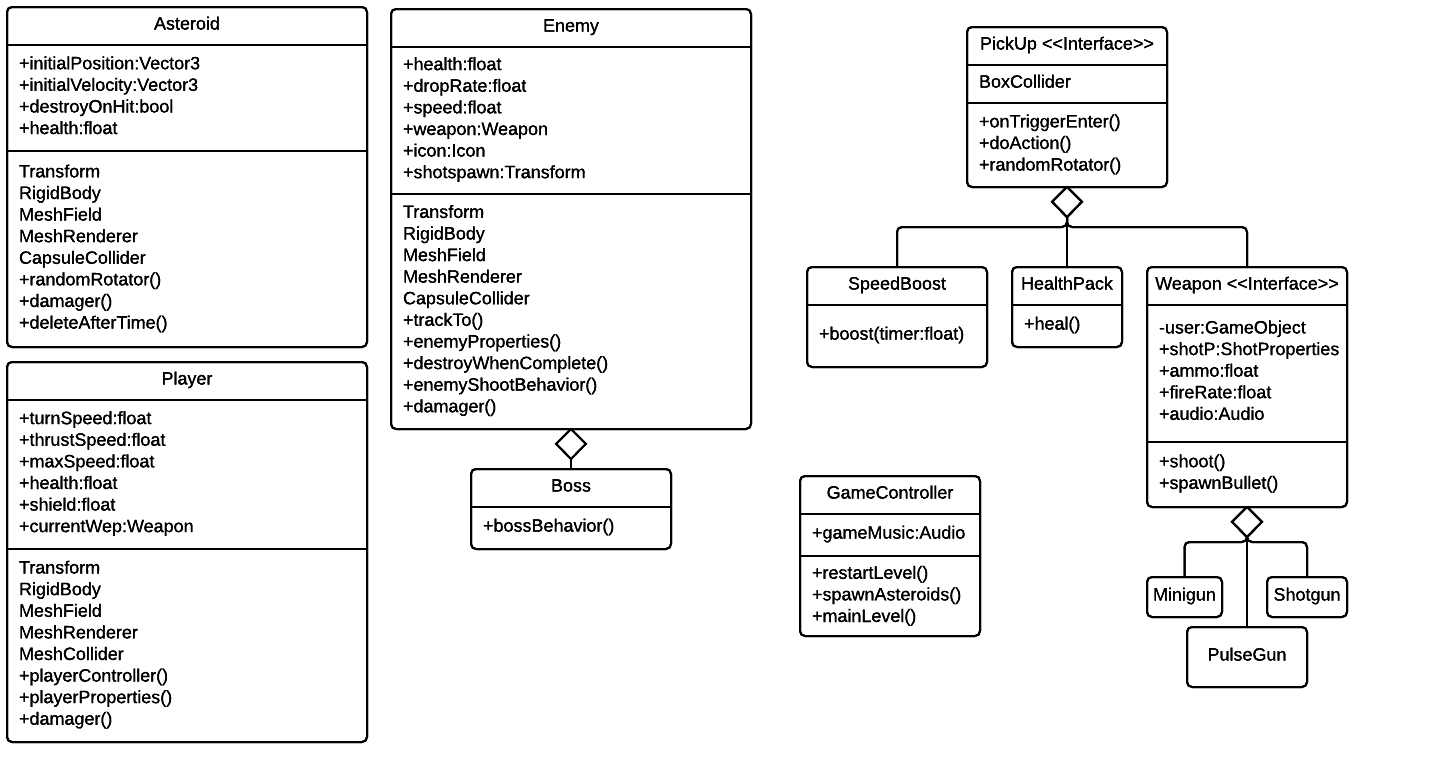
\includegraphics[width=7.3in]{FinalUMLHorizontal.png}
\caption{UML Diagram} \label{UML}
\end{figure}

\subsection{State Diagram}
Figure \ref{StateDia} describes the transitions between various scenes and menus in the game. Each state corresponds to either a Unity scene or a GUI child menu.

\begin{figure} [H]
\centering
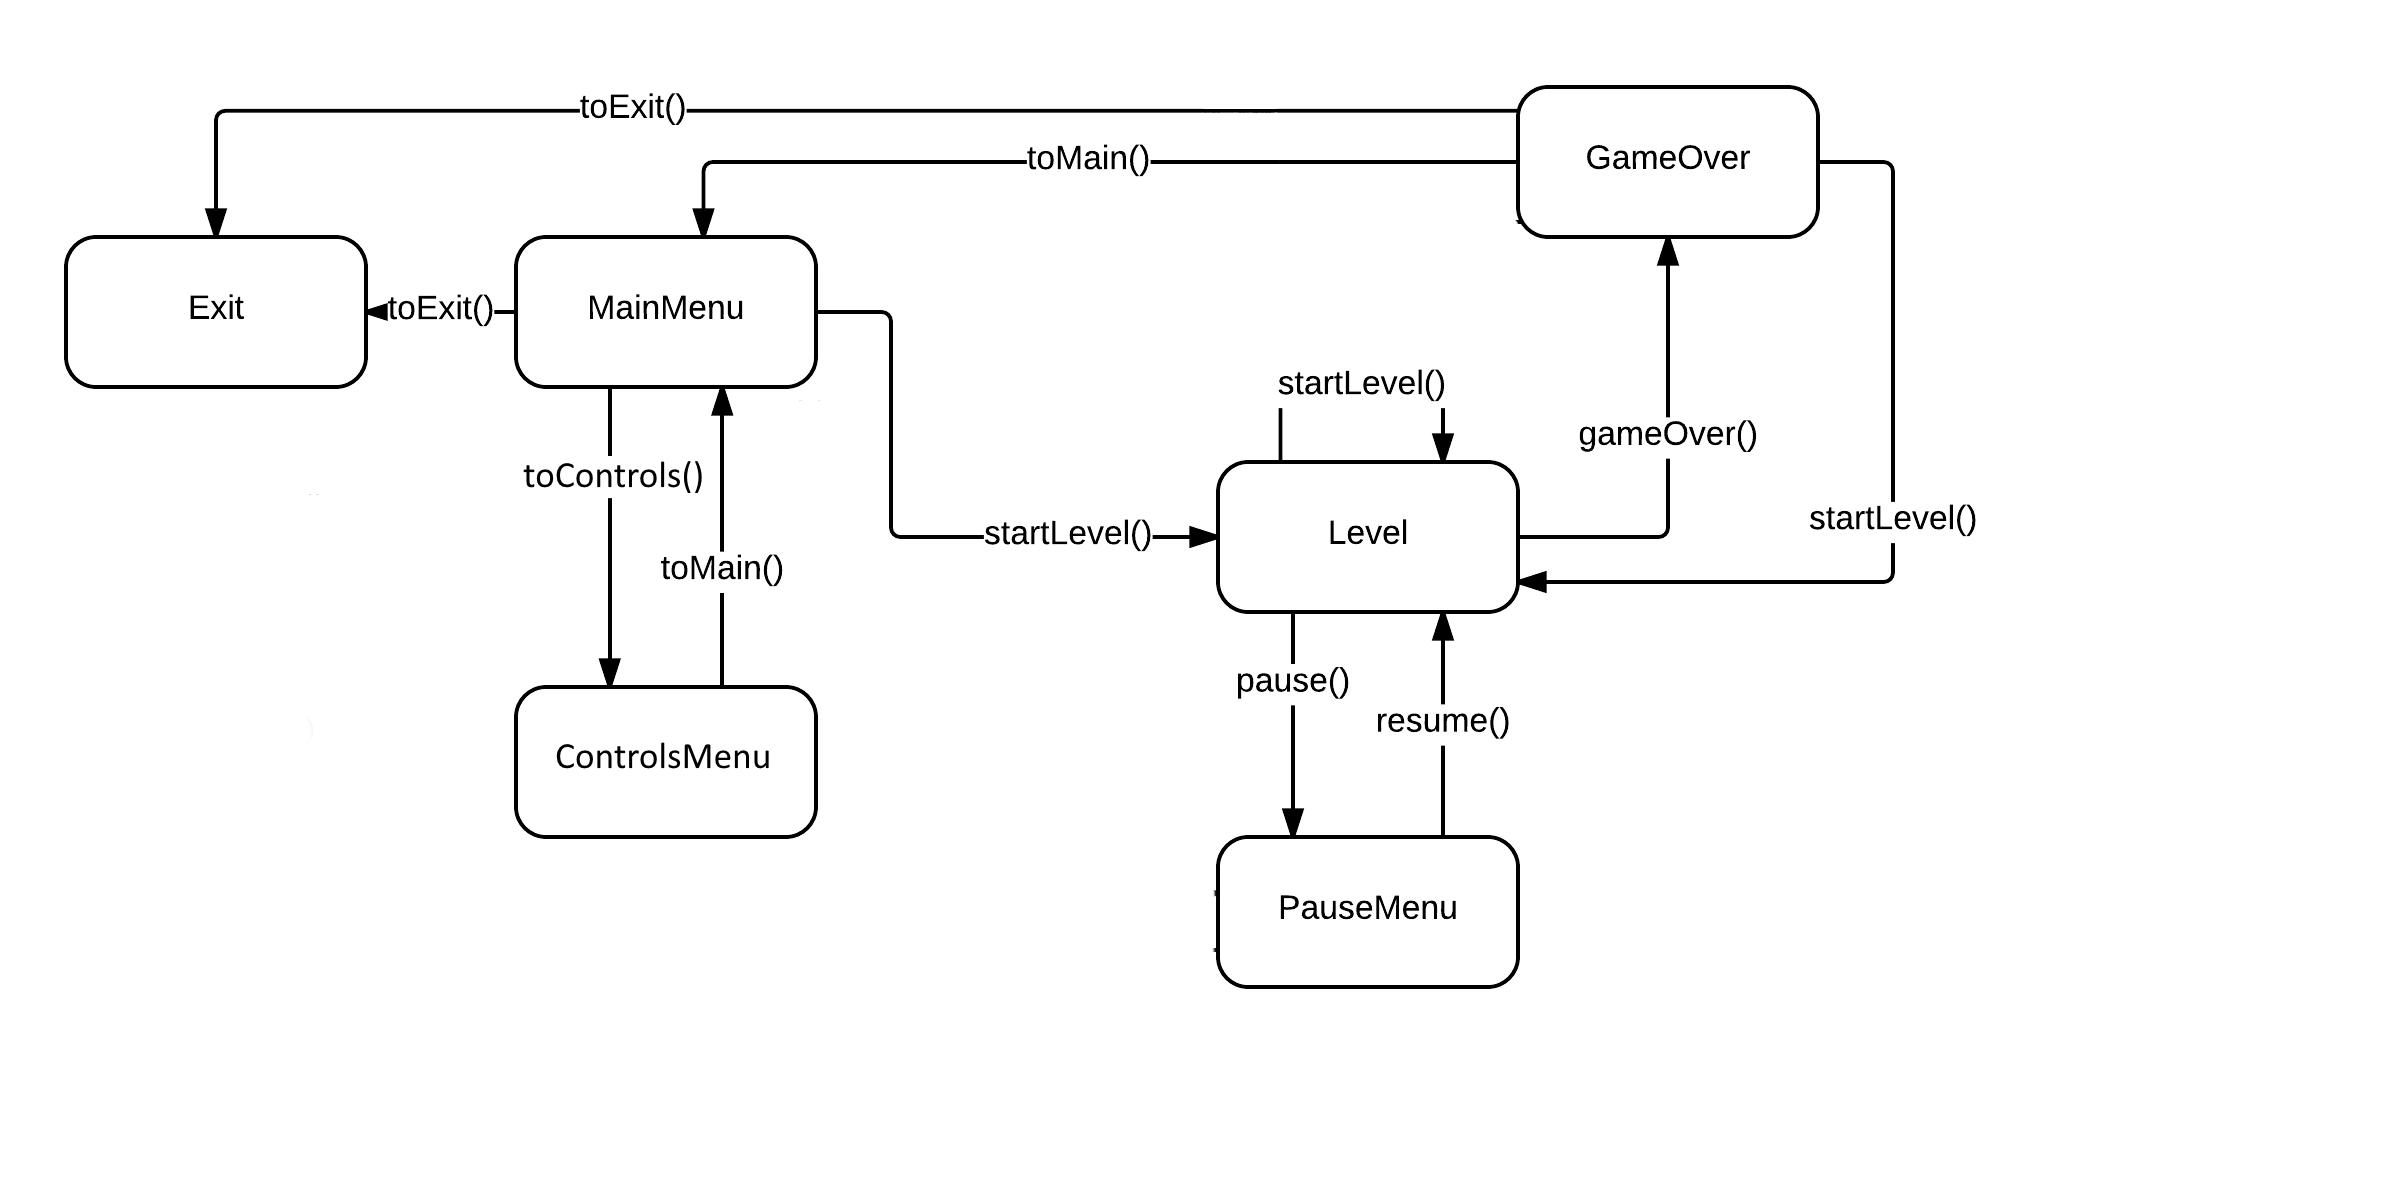
\includegraphics[width=7in]{PewPewStateDiagramFinal.png}
\caption{State Diagram} \label{StateDia}
\end{figure}

\hs {\bf Testing plans}: The group members will play the game every step of the way to make sure that the individual additions to the project are functioning as expected. Once there is a version of the game that allows a player to navigate an environment and fight basic enemies, the group will reach out others to play it and give feedback in the form of a simple survey. 

\section{Gameplay Design} %GAMEPLAY DESIGN
\label{sec:GPdesign}

Games are dynamic pieces of software that focus on delivering exciting or interesting experiences to players, gameplay design is as important as backend design. What follows is the basic design for the aspects of the gameplay that the player will see for our current iteration of the game.

\subsection{Player} %Player

	{\bf Player controls: }The player controls a small spaceship, and navigates through a space environment. As seen in Figure \ref{Controls}, the player will move with the WASD keys; pressing a key will cause the ship to rotate to and accelerate in that direction.  Shooting will be controlled by the arrow keys on the keyboard. Pressing an arrow key will cause shots to be fired in that direction. Since movement and shooting are separate, the player may move in one direction and fire in another.  The player can also pause the game with the escape button. The controls are intended to transfer over to a controller relatively easily, so the player may control moving and shooting with the left and right analog stick respectively. The controls diagram is located at Section 5.7 of this document.

	{\bf Player Movement:}	As stated above, the player presses either the WASD keys or the left analog stick to begin rotating and accelerating in that direction. Rotation has a maximum speed, so quickly changing direction causes the ship to veer in a small circle as it rotates to face the intended direction. Acceleration speed will not be instantaneous and the player will not stop automatically, in order to simulate a sense of weight and the lack of friction in space. The ship will perform these actions quickly enough that controlling the ship feels responsive to the player.

	{\bf Player Shooting:} Player shooting functions similarly to player movement in terms of input. By pressing the arrow keys or on the right analog stick, the player will shoot in the respective direction. The player's ship has a rotating gun attached to it, which allow the player to aim and shoot in any direction regardless of current movement. However, there is no rotation time for the gun on the player's ship, so the gun will shoot instantaneously in the direction that is being pressed. Be default the player's ship shoots a rapid fire laser, which will allow the user to get comfortable with shooting without having to worry about missing or wasting ammo. Various weapon pickups can be used to modify how the player's weapon shoots (detailed in Section 5.3). The control method will remain the same for all weapons so the player does not have to worry about learning different controls for each weapon.

	{\bf Player ship:} The player's ship will have its own health and shield values. The shield will be a rechargeable defense that will be able to absorb a number of shots before the players ship takes permanent health damage. Recharging of the shield will occur over time after a few seconds of avoiding damage. The ship's health is the amount of damage the ship can sustain before it explodes and the player loses. It will not regenerate automatically like the shield, but items will be able to restore it.

\subsection{Enemies} %Enemies

	\hs {\bf Enemies: } The main goal of enemy ships is to kill the player ship. They will have two main types of AI that will decrease the predictability of enemies and prevent the player from staying still for too long. \\

	{\bf Standard Shooting:} Standard shooting is when the enemy just shoots straight in the direction it is currently facing.  This is usually in the direction of the player. \\

	{\bf Predictive Shooting:} Predictive shooting is when the enemy uses a special method to predict where the player will be when the shot reaches it. This creates an effect where the enemy is shooting in front of the player so that the shot hits the player most of the time. \\

	{\bf Patrolling:} In order to patrol the enemies will set their spawn point to ``home''. Every time they are to far away from the player to track them, they will return ``home" and circle around it until the player comes back in to range. \\

	{\bf Enemy Type One:} The first type of enemy tracks directly toward the current location of the player while it moves. It will try to stay a small ways away from the player to avoid colliding with them. This enemy type has a high possibility of shooting at a fixed time interval, using standard shooting. \\

	{\bf Enemy Type Two:} The second type of enemy will follow the player more closely than the first type while also trying to get in front of the player. This type uses standard shooting with medium damage shot, firing less frequently than the first type. \\

	{\bf Bosses:} Bosses will give the player a final challenge before ultimately reaching the end of the game and winning. Bosses will shoot large amounts of projectiles to making dodging difficult for the player. Additionally, the boss will have a predictive shooting projectile to increase the difficulty further. Finally, bosses will have a larger amount of health than the average enemy. Defeating a boss will end the game and display a win screen. \\

\subsection{Weapons} %Weapons

	{\bf Weapons:} Weapons are implemented through the Unity prefab system. By default, the player is given a low-damage, high rate-of-fire red laser weapon that they can change by finding a weapon pickup which drops off enemies. Once the player makes contact with the pickup, their current weapon is destroyed and the new weapon is loaded for the player. All non-default weapons have a limited amount of ammunition, and once their ammo is depleted, the weapon is destroyed and replaced with the default weapon.

	\begin{enumerate}
	\item {\bf Shotgun:} The shotgun has the same damage and rate of fire as the default weapon. However, every shot of the shotgun fires five bullets in a short, fixed spread, rather than one bullet straight ahead. Has 50 ammo.

	\item {\bf Pulse Gun:} The pulse gun is a high damage, low rate of fire gun that shoots one large pulse of 70 green bullets in the direction the player presses. Bullets fired by this gun do not destroy themselves when colliding with an entity, allowing for a "piercing" effect. Has 10 ammo.

	\item {\bf Minigun:} The minigun has a much faster rate of fire than the default gun. However, its damage is half of the default gun's per shot and the exact direction the bullets will be fired in has a variance, not guaranteeing accuracy. Has 400 ammo.
	\end{enumerate}


\subsection{Levels/Objects} %level

	{\bf Pick-ups:}  There will be pick-ups available to the player throughout the game, dropping from enemies. Most pick-ups will change some attribute of the player ship, such as giving the player an alternative weapon, a temporary speed increase, or restoring the player's health. Additionally, there is another pickup that will spawn a follower ship that will follow the player ship around that map and shoot at nearby enemies. Some pick ups will be displayed in part of the UI (Section 5.5), such as the speed boost meter.

	{\bf  Items:} Items are intended to either provide a permanent boost to the player attributes (such as speed or maximum health), or add an effect that the player can activate by pressing a button, such as a time bomb that would slow down enemies and asteroids when activated, making them easier to dodge. There are currently no items implemented in the game, but could be included in the future. 

	{\bf Level design:} The level consists of a circular arena. There is a circular border around the playing field that the player will be shot at if crossed. Enemies spawn in waves inside the arena but outside the player's view. Asteroids spawn in and around the arena. As the player destroys waves of enemies, new larger waves will spawn. After completing a set number of waves, the boss will spawn in the arena.

	{\bf Star Field and Background:} The background will be a two dimensional tile that can be replicated across the screen to create a smooth, endless field of stars. The star field layered on top of the background image is particle effect conisting of small drifting particles that will move across the screen. The multilayering will add a three-dimensionality to the background and keep the background from being static.

	{\bf Asteroids:}  Asteroids will be obstacles that will fly across the screen, dealing damage to anything they collide with. This forces players to be more aware of their surroundings or risk dying and gives them another danger they must avoid. Asteroids have no set allegiance and can collide with each other and enemy ships. Asteroids will spawn in random locations outside the player view with a random initial velocity and direction. Asteroids will travel until they either collide with a ship, get shot by the player, or travel outside of the level boundaries.

\subsection{User Interface} % UI

	{\bf Radar:} The radar will be displayed in the bottom left corner. It shows the player the location of all enemies, pick-ups, and asteroids in the immediate surrounding area of the player. In addition, it also represents the direction of all enemies not shown in the immediate area with a symbol on the edge of the radar, assisting the player with locating all enemies in a wave.

	{\bf HUD:} The player has access to a Heads-Up Display in the bottom right corner, which displays vital information, such as the player's health, shield, currently equipped weapon, ammo remaining, the current wave, and the number of enemies left in the wave. The HUD will also display if the player is currently under the effects of a speed boost and how much time is remaining on their speed boost.

	{\bf Menus:} Menus in the game consist of a selection of several buttons that the user can select with the cursor to navigate through different game states. The primary menu is the main menu, which allows the user to start the game, navigate to the controls menu, or exit the application. The controls menu gives a brief game discription and shows the controls, with an option to return to the main menu. Additionally, there is a pause screen that appears when the player pauses in game that shows a few different controls that can be used to resume or restart the game.

\subsection{Art} %Art

	\hs {\bf Story:} The Player is an explorer trying to reach the other side of the Universe to meet aliens that sent a treasure map to earth. The Player keeps in close contact with General Weathersbee who guides them to the last known location of the aliens. 

	{\bf Art/models:} The assets and models used in this project will mostly be free from the Unity store. Our group created some of the simple icons, used in the radar and the HUD. Some of the assets are combined and blended together to create a unique model specifically for this game. For example, there is a gun from one asset pack combined with a ship from another pack to create a new ship type. There is a black with stars background for the main level, with a moving star field overlay. The other scenes have varying space themed backgrounds, with the same star field. The font Huxley is used uniformly through out the game to tie the scenes together.  

	{\bf Music/ sound:} Sound effects and music will be retrieved from the Unity store and other sites that allow people to download and use their music for non-commercial purposes. The music is upbeat and fast paced to set the tone of the game. The sound effects will mostly be explosions and gun sounds. For example the laser gun will have a "pew pew pew" sound. 


\subsection{Controls Diagram}

\begin{figure} [H]
\centering
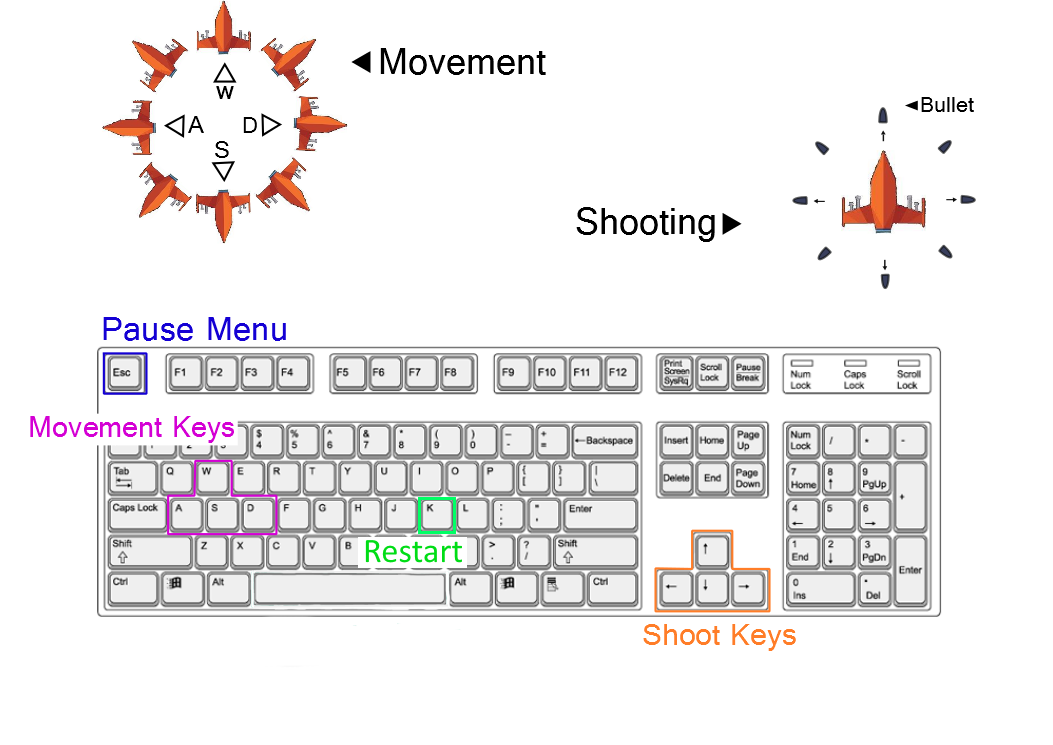
\includegraphics[width=6.3 in]{ControlDiagramFinal.png}
\caption{Controls Diagram} \label{Controls}
\end{figure}


\section{Implementation} %IMPLEMENTATION
\label{sec:history}
This section describes the completed work, current status, and future plans that are to be included to the project.

\subsection{Work Completed}

\hs The Unity website offers in-depth tutorials on how to create basic games using the Unity engine. We have completed two specific tutorials in preparation for this project: The “Beginner” rated project, entitled “Space Shooter”, and the “Intermediate” rated project, “Project: Stealth”.

  The “Space Shooter” tutorial introduced us to the basics of Unity, and explained how to use the engine to create a top-down, two-dimensional space shooter game using given assets, including a three-dimensional ship model, a provided background, and models for asteroids and enemy ships. It also provided sample scripts to use for the completed game, written in $C\#$. The completed project spawned varying waves of asteroids that the player would have to either shoot or dodge, with a score counter incrementing every time the player shot an asteroid and the game ending when the player took damage from colliding with an asteroid and dying.

 The “Project: Stealth” tutorial went into much more depth than the “Space Shooter” tutorial, and guided us through making a fully functional three dimensional stealth-based game. Using provided assets, the tutorial showed us how to use animations to change collisions, enemy AI that reacted to various events that the player had some limited control over, and advanced $C\#$ scripting work that went into more detail than the basics in the “Space Shooter” tutorial. The finished project was a fully functional game in which the player would attempt to reach the end of a level without alerting various AI guards.

  We intend to use many of the elements presented in both of these tutorials as building blocks in our own game. From the “Space Shooter” tutorial we intend to use the fundamental concepts presented in the tutorial, namely scripting, collisions, and two-dimensional top-down shooter action, in our product. From the “Project: Stealth” tutorial we intend to use some of the overall concepts, such as enemy artificial intelligence and events occurring in response to our game state in our product.

\subsection{Current Status}

In the current state of the project many of the functional goals have been accomplished. By the academic festival we aimed to have at least five different pick-ups, a loss condition, a boss with a corresponding win condition, and a single level. We have finished all of these goals and created a playable and winnable game. Additional features that have been added during development include a predictive shooting method, a follower, and independently rotating guns attached to the player and boss ships. Due to the lack of time, the game's level structure was modified from a multi-level adventure to wave-based gameplay in an arena.

\subsection{Future Work}
Since our project is in a complete state, anything added would be to expand or enhance the game. That being said, if we had more time to work on this game there are a few things that we could work on:
\begin{itemize} 
	\item {\bf Update Assets:} Finding new assets or learning to create our own assets would be helpful for creating a more consistent art style. As well as creating a more unique game that does not have the same assets as many other low budget space games.  
	\item {\bf Update AI:} Adding more sophisticated and challenging AI would be a way to add difficulty to the game. It would also smooth out the movement of the enemies making them less jumpy and less predictable. 
	\item {\bf Adding Menus:} Menus that add a  ship selection, achievements or  options like difficulty, would increase peoples desire to replay of the game. For example if the way to unlock more ships was by completing achievements, people would have to play the game multiple times if they wanted to play with a new ship.
	\item {\bf Adding Levels:} More levels would vary the game play more and make it possible to incorporate our story in to the game. 
\end{itemize}



%\section{Timetable}
%\label{sec:time}
%Figure \ref{Time} describes the planned development cycles for creating the game.

%\begin{figure} [H]
%\centering
%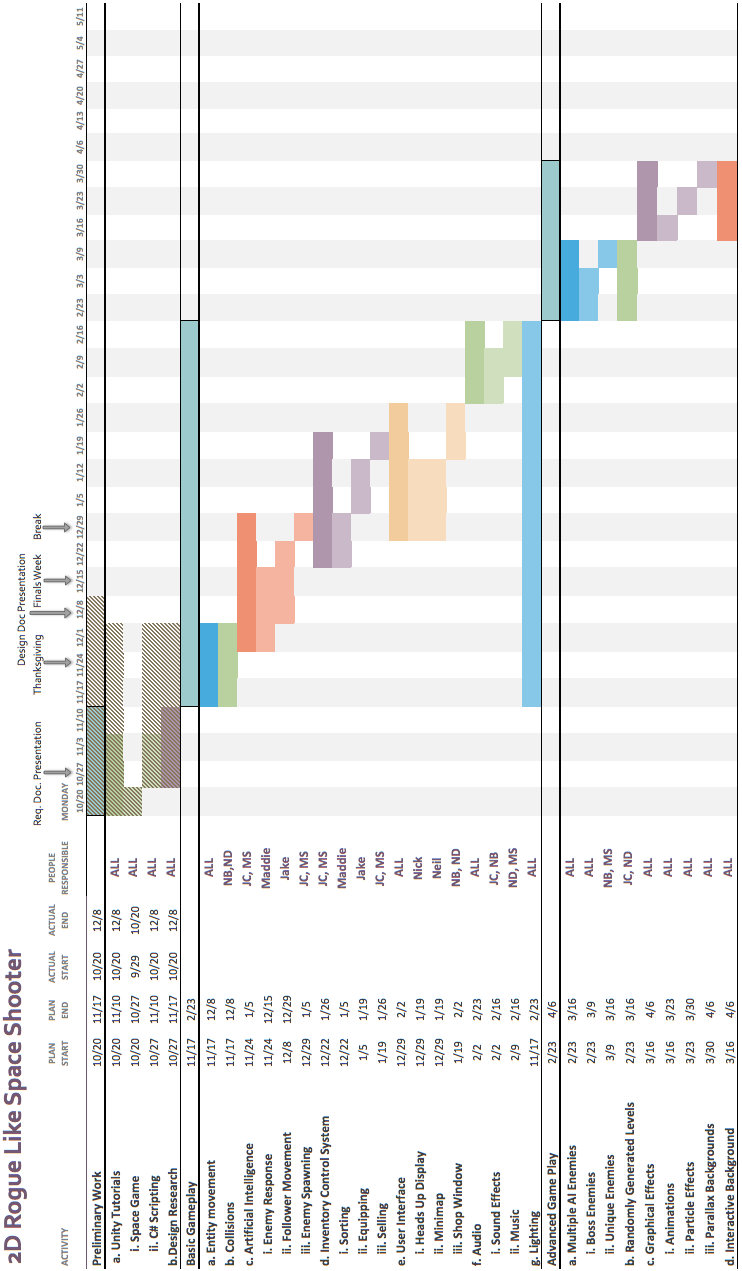
\includegraphics[width=4.3 in]{TimeTableDec.png}
%\caption{Current Time Table} \label{Time}
%\end{figure}


\newpage
%\section{References}
%\label{sec:ref}

\begin{thebibliography}{99}

\bibitem{History} Ringo, D. History of Gaming: A Look at How It All Began. Public Brodcasting Service, n.d. Retrieved October 20, 2014, from PBS: http://www.pbs.org/kcts/videogamerevolution/history. 

\bibitem{Tutorials} Tutorials. Unity Technologies, n.d. Retrieved October 15, 2014, from Unity: http://unity3d.com/learn/tutorials/modules.

\bibitem{C} Creighton, R. Unity 4.x Game Development by Example Beginner's Guide, 3rd ed. Packt Publishing, Birmingham, UK, 2013.

\bibitem{Edgar} Edgar, T. Latex-slides. Department of Mathematics Pacific Lutheran University, Tacoma, WA, September 2011. PDF. 

\bibitem{Rogue} A Brief History of Roguelikes, Kill Screen Daily. Retrieved November 14, 2014 from Kill Screen Daily, INC: http://killscreendaily.com/articles/brief-history-roguelike/.

\bibitem{PCG} Procedural Content Generation Wiki. Retrieved December 4, 2014 from: http://pcg.wikidot.com/.

\bibitem{Cadet} Cadet, H. A Brief History of C Sharp.  N.p., n.d. Retrieved November 13, 2014 from Hernando Cadet Technology:  http://www.hernandocadett.com/content/brief-history-c-sharp/.

\bibitem{E} Elias, H. Perlin Noise. Retrieved December 6, 2014 from: http://freespace.virgin.net/hugo.elias/models/m\_perlin.htm.

\bibitem{Moles} Moles, S. How Does Unity Use $C\#$ as a Scripting Language? N.p., n.d. Retrived: November 13, 2014 from Game Development Stack Exchange: http://gamedev.stackexchange.com/questions/51350/how-does-unity-use-c-as-a-scripting-language.

\bibitem{Ogre} About Object-Oriented Graphics Rendering Engine. Retrived November 2014 from Torus Knot Software: http://www.ogre3d.org/about/

\bibitem{Guide} Stevens, P. and Tenzer J. GUIDE: Games with UML for Interactive Design Exploration. 
{ \it Laboratory for Foundations of Computer Science School of Informatics}. Retrived November 16, 2014 from University of Edinburgh: http://homepages.inf.ed.ac.uk/perdita/guide.pdf.

\bibitem{UML} UML for games. November 2003. Retrived November 16, 2014 from GameDev.Net LLC: http://www.gamedev.net/topic/192120-uml-for-games/

\bibitem{A} Patel, A. Introduction to A*. Red Blob Games, 1997. Retrived November 18, 2014 from Stanford University: http://theory.stanford.edu/~amitp/GameProgramming.
 
\bibitem{GDD} Effectively Organize Your Game's Development With a Game Design Document. Tutsplus. Gamux. Envato, November 11, 2011. Retrived November 18, 2014 from Tutsplus: http://code.tutsplus.com/articles/effectively-organize-your-games-development-with-a-game-design-document--active-10140. 


\end{thebibliography}

\newpage

\section{Glossary}
\label{sec:gloss}

{\bf{AI}} - Artificial Intelligence, in our case directing the actions of the NPCs. \\
{\bf Boss} - A unique hostile entity that appears at the end of a level. \\
{\bf Entity} - An object that can interact with other objects in the game. \\
{\bf Field of Play} - The area in which a player will interact with obstacles, enemies, and other events. \\
{\bf HP} - Health points, a measure of the players health level often represented as either a fraction or bar. \\
{\bf HUD} - Heads Up Display, the in game area of the screen that displays player statistics like health or ammo left. \\
{\bf Level} - A collection of similarly challenging fields of play culminating in a boss. \\
{\bf NPC} - Non Player Characters, e.g., any enemies or passive characters that act in the game that are not controlled by the player. \\
{\bf Parallax} - The effect whereby the position or direction of an object appears to differ when viewed from different positions, e.g., elements far from the camera appear to move more slowly than foreground elements. \\
{\bf Prefab} - A function supported by Unity that allows for predefined object specification and quick entity instantiation. \\
{\bf Ramming} - When one entity attacks another through direct collision. \\
{\bf Roguelike Game} - A game that is distinct because of two important characteristics:
Has highly randomized gameplay with a large amount of replayability. 
Permanent death, meaning if the main protagonist dies, the game ends and the player must restart from the beginning. \\
{\bf Sprite} - The image that represents entities in the game. \\
{\bf Unity} - The primary game engine we will be using. \\
{\bf Unity3D} - The software kit used to develop games in Unity. \\
{\bf Usable Items} - Items the player can use by pressing the use item key. \\



\end{document}



